\subsection{Distributed Memory Model}
Attributes are numerical quantities associated with a topology. For
example, common attributes may be vector valued wind directions computed by an
atmospheric modeling algorithm at the vertices of a triangulated 2D
topology. Another algorithm may have also simulated air temperature,
a scalar attribute, at the centroid of cell volumes specified by a 3D
topology. Attributes have their own dimensionality which is not
necessarily equal to the dimension of the topology.

The local topology cache and external attribute mechanism defines a
distributed memory model for datasets registered with \sciwms{}. Given
a request for the visualization of a attributes pertaining to a region
of interest, the visualization pipeline consists of first computing
the sample locations withing the region of interest, using the
implicit representation for \cgrid{} and \rtree{}s for \ugrid{}
topologies, then fetching the corresponding external attributes. For
rendering, the sample connectivity within the area of interest is
reconstructed from the connectivity array which is utilized for
interpolation.
%% The local topology cache and external attribute mechanism defines a
%% distributed memory model for datasets registered with \sciwms{} as
%% visualized in figure~\ref{fig:sciwms_mem_model}. The grid on the left,
%% depicts a regular grid stored locally to \sciwms{}. A possible region
%% of interest is highlighted by the dashed red square. Attributes are
%% stored externally by multiple institutions and are exposed to
%% \sciwms{} in such a way as it can be visualized using the table on the
%% left of the figure. Different attribute layers are represented by the
%% rows of the table while columns correspond to memory locations of
%% attribute values associated with the topology. %% In this example,
%% attributes associated with positions within the region of interest
%% correspond to memory locations highlighted by the red cells in the
%% table. Given the request for a rendering of an attribute layer(s),
%% \sciwms{} dispatches a request for externally hosted numerical data
%% necessary to render the region of interest.
%% \begin{figure}[ht!]
%%   \centering
%%   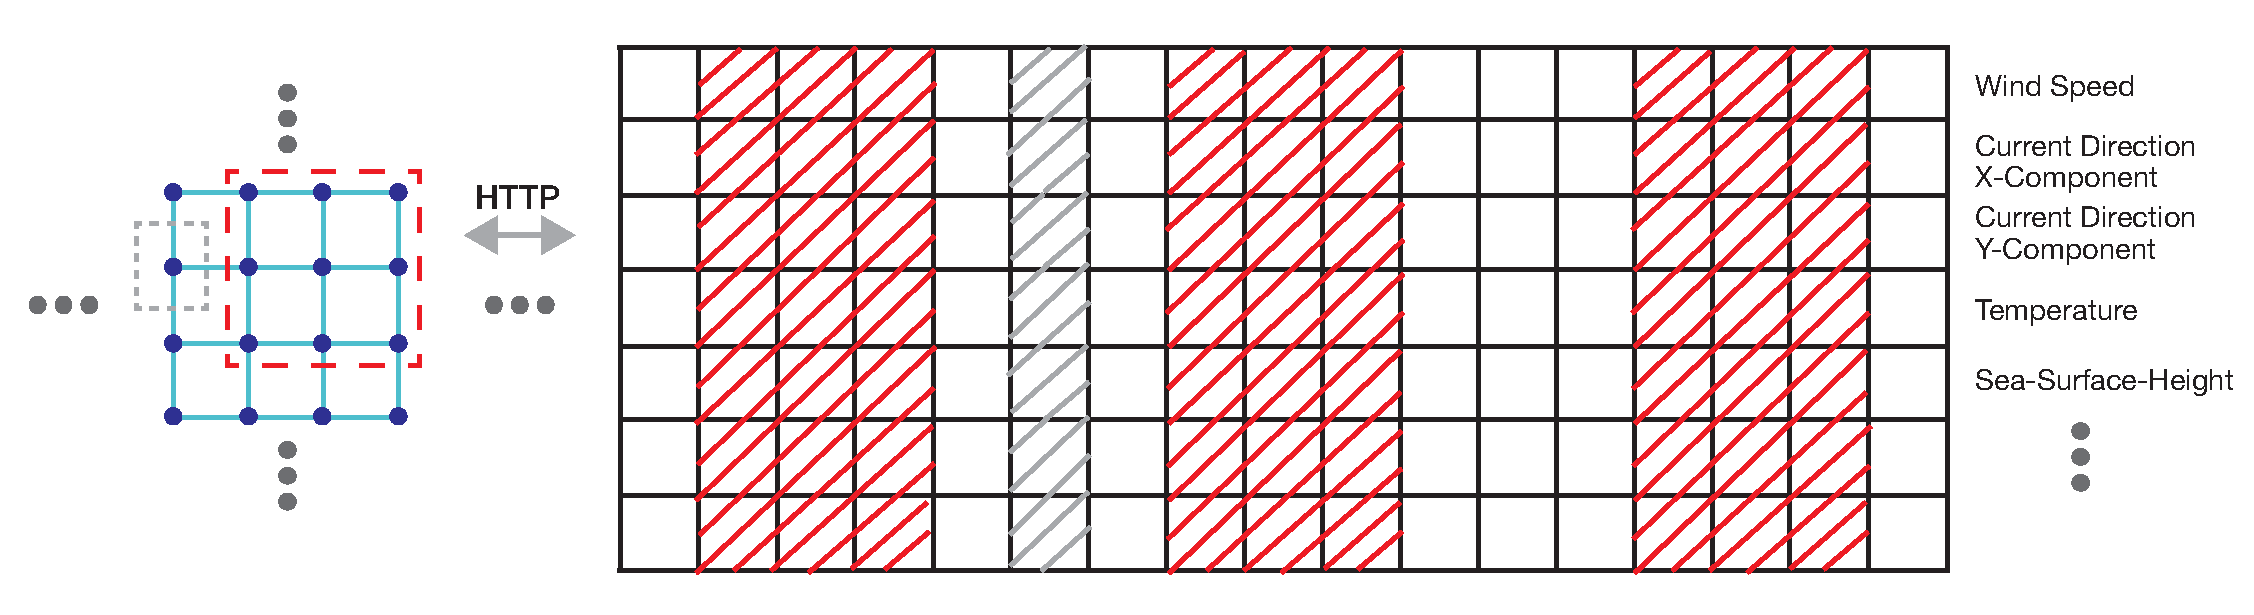
\includegraphics[width=\textwidth]{../figs/topology_memModel}
%%   \caption{The \sciwms{} distributed memory model.}
%%   \label{fig:sciwms_mem_model}
%% \end{figure}
